An overview of the workflow is shown in \autoref{fig:workflow}. The data analysis includes many heterogeneous steps using different bioinformatics programs and scripting languages. To ensure reproducibility and transparency, we used the Snakemake workflow management system,~\cite{molderSustainableDataAnalysis2021} and all the code is hosted in a public repository on GitHub (\url{https://github.com/currocam/BiRC-Thyme}).\\

% Add image 
\begin{figure}[ht!]
    \begin{center}
        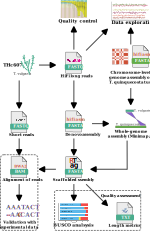
\includegraphics[width=0.9\textwidth]{gfx/methods.pdf}
        \caption{Workflow of the data analysis}   
        \label{fig:workflow}
 
    \end{center}
\end{figure}  

\section*{Quality Control of raw reads}

We computed the theoretical coverage based on cytometric estimates of the genome size of \textit{T. vulgaris}.~\cite{PlantDNACvalues}\\

We used two automated quality control tools: FastQC~\cite{BabrahamBioinformaticsFastQC}, a well-known general program, and LongQC,~\cite{fukasawaLongQCQualityControl2020} a specific program for genomic datasets generated by third-generation sequencers. We also trimmed adapters from \ac{HiFi} reads using LongQC.~\cite{fukasawaLongQCQualityControl2020} \\

\section*{Exploratory analysis of long reads and reference genome}

As part of our exploratory analysis, we aimed to assess how well the long reads of \textit{T. vulgaris} align to the reference genome of \textit{T. quinquecostatus}, as this will be critical in evaluating the confidence in the final assembly.  \\

We retrieved the \textit{T. quinquecostatus} genome assembly published by Sun \etal from NCBI (Accession identifier: PRJNA690675).~\cite{sunChromosomelevelAssemblyAnalysis2022} We aligned a subset of the \textit{T. vulgaris} long reads to the \textit{T. quinquecostatus} assembly using Minimap2~\cite{liMinimap2PairwiseAlignment2018} with default parameters for \ac{HiFi} sequencing. To construct the subset of long reads, we filtered by quality, keeping the sequences corresponding to the best 5\% (measured in nucleotides) using the specific program for this purpose Filtlong.~\cite{RrwickFiltlongQuality}\\

We measured the percentage of mapped reads, the distribution of alignment lengths, and the coverage using samtools.~\cite{danecekTwelveYearsSAMtools2021} We studied the distribution of the mapped reads across the \textit{T. quinquecostatus} genome. We computed the number of mapped reads in 1000-long windows, $Y = [ y_1, y_2, \dots, y_w]$ to accomplish this. We decided to use the number of mapped reads instead of counting the mapped positions. The latter results in a less informative Normal distribution due to the Central Limit Theorem.~\cite{whitlockAnalysisBiologicalData2015}\\

We propose that mapped reads can be accurately modeled as a Zero-inflated Poisson process, as shown in Equation \eqref{eq:zip}. \\

\begin{equation}
\label{eq:zip}
Y = \begin{cases} 0, & \textrm{with probability } p \\ \textrm{Poisson}(\lambda), & \textrm{with probability } 1-p \end{cases}
\end{equation}

We estimated the missing parameters of the model, $\lambda$ and $p$, through Bayesian inference. We examined the posterior distribution of $\lambda$ and $p$ to evaluate the model's goodness of fit. In the discussion section, we provide a potential explanation of the implications of the Zero-inflated Poisson model.\\

We computed the posterior distributions based on very uninformative priors and a \ac{MCMC} sampler with a single chain and a small number of iterations: 200 in the adaptive phase and 500 in the sampling phase. The entire model specifications are shown in Equation \eqref{eq:model}. We implemented the model using Turing, a probabilistic programming library.~\cite{DBLP:conf/aistats/GeXG18}

\begin{subequations}
\label{eq:model}
\begin{align}
Y \sim \textrm{ZIPoisson}(p, \lambda) \label{eq:model1}\\
p \sim \textrm{Uniform}(0, 1) \label{eq:model2}\\
\lambda \sim \textrm{Gamma}(1, \alpha)  \label{eq:model3}\\
\alpha = \textrm{Ave}(Y) \label{eq:model4}
\end{align}   
\end{subequations}
%Add title with cursive words

\section*{De novo assembly}\label{sec:denovo}

A \textit{de novo} assembly of \textit{T. vulgaris} was available. This assembly was made from the long reads using Hifiasm~\cite{chengHaplotyperesolvedNovoAssembly2021} with default parameters. We compared the genome size of the assembly, obtained with sequenced data,  with cytometric estimations.~\cite{PlantDNACvalues}

\section*{Homology-based assembly scaffolding}\label{sec:scaffold}

Using the program RagTag,~\cite{alongeAutomatedAssemblyScaffolding2022} we scaffolded the \textit{de novo} assembly. In general terms, the process consisted of: 
\begin{enumerate}
    \item Perform a whole-genome alignment of \textit{T. vulgaris} against \textit{T. quinquecostatus} assembly using Minimap2. 
    \item Order and orient the contigs into longer sequences (scaffolds) according to the alignment. 
    \item Join adjacent contigs of \textit{T. vulgaris} with gaps of inferred size. 
\end{enumerate}

As established by Alonge \etal~\cite{alongeAutomatedAssemblyScaffolding2022}, RagTag infers the gap size between two adjacent sequences, $\textrm{seq1}$ and \textrm{seq2}, according to Equation \eqref{eq:infergapsize}

\begin{equation}\label{eq:infergapsize}
\textrm{gapsize}  = \left(\textrm{aln2}_\textrm{rs} - \textrm{aln2}_\textrm{qs}\right) - \left(\textrm{aln1}_\textrm{re} - \textrm{aln1}_\textrm{qe} + \textrm{len}(\textrm{rs}\right)
\end{equation}

where $\textrm{rs}$, $\textrm{re}$, $\textrm{qs}$ and $\textrm{qe}$ denote the start and end position of the alignment in the reference and query sequence, respectively. If the gap size is smaller than 100 bp or bigger than 100,000 bp, the inserted gap is forced to be 100 bp, indicating an unknown gap according to the AGP specification.~\cite{AGPSpecificationV2} 

\section*{Assembly quality assessment}

Assessing genome assemblies' quality is a crucial step in this analysis. There are different approaches to evaluate assembly quality, including length-based metrics and annotation-based metrics.~\cite{mokhtarLargescaleAssessmentQuality2023} While a comprehensive assessment of assembly quality is beyond the project's scope, we have focused on two commonly used metrics: N50 and BUSCO (Benchmarking Universal Single-Copy Orthologs).~\cite{manniBUSCOAssessingGenomic2021} \\

N50 is a length-based metric that provides an estimate of contiguity. It represents \enquote{the shortest fragment size at half the genome size}.~\cite{mokhtarLargescaleAssessmentQuality2023} A higher N50 value indicates better contiguity and suggests that the assembly has longer contigs or scaffolds. BUSCO, on the other hand, is an annotation-based metric, and it assesses the presence or absence of a set of highly conserved and universal orthologous genes. \\

We used assembly-stats~\cite{SangerpathogensAssemblystatsGet} for collecting technical metrics, among them N50. We ran BUSCO analysis using the datasets eudicots\_odb10 (2023-04-05) and eukaryota\_odb10 (2023-04-05). However, we report only the former's results since it is more specific for thyme.\\



\section*{Mapping short Illumina reads to scaffolds}\label{sec:illumina}

The demultiplexed Illumina reads of three specimens of \textit{T. vulgaris} and two of \textit{Satureja montana} were available (see \autoref{tab:illumina_samples}), including reads from the same individual sequenced using \ac{HiFi}. These sequences were used to validate the assembly with independently obtained data. \\

\begin{table}[h]
    \begin{minipage}{\linewidth}
    \renewcommand\thefootnote{\thempfootnote}
    \centering
    \begin{tabular}{@{}llll@{}}
    \toprule
    Sample Id & Scientific name & Location     \\ \midrule
    THc607\footnote{The same individual used to generate the genome assembly}    & \textit{T. vulgaris}   &  Cefe Montpellier  \\
    THb134    & \textit{T. vulgaris} & Mont St. Baudille   \\
    THa252    & \textit{T. vulgaris}& \\
    SAa062    & \textit{S. montana} & Cabanne     \\
    SAa046    & \textit{S. montana}  & Roc Blanc    \\ \bottomrule
    \end{tabular}
    \caption{Specimens sequenced with Illumina and mapped to the \textit{T. vulgaris} assembly}
    \label{tab:illumina_samples}
    \end{minipage}
    \end{table}

Reads were sequenced using a targeted enrichment protocol. Two different hybridization conditions were employed before the construction of sequencing libraries.\\
\begin{enumerate}
    \item Hybridization 1 is a standard capture protocol that, according to the manufacturer, supports up to 15\% nucleotide divergence between the bait's (biotinylated oligonucleotide probes) nucleotide sequence and the captured genomic DNA. 
    \item Hybridization 2 is a more stringent procedure developed for a more specific capture (details for the specific steps are in the supplementary information and protocols of Bataillon \etal~\cite{bataillonGenotypePhenotypeGenetic2022}). The expected nucleotide divergence supported between the bait and the genomic target is much lower and roughly estimated to be within five percent of nucleotide divergence to \textit{T. vulgaris} (used for the original bait design).
\end{enumerate} 

We aligned these reads to the scaffolded assembly using BWA-MEM with default parameters.~\cite{liAligningSequenceReads2013} Although this report did not include experimentation with different parameters, it was conducted to optimize the results. Better outcomes were achieved by assigning higher penalties to SNPs (Single Nucleotide Polymorphism) and indels than the default settings. However, for a more appropriate comparison between species, default parameters were used in this study.\\
